% Report: at most 8 pages (task.md). Build: cd report && latexmk -pdf report.tex
% Figures: report/figures/ (python report/make_figures.py) and output/final_sweep/plots/.
\documentclass[10pt,a4paper]{article}
\usepackage[margin=2cm]{geometry}
\usepackage{graphicx}
\usepackage{booktabs}
\usepackage[section]{placeins}   % figures stay inside their own section
\usepackage{amsmath}
\usepackage{enumitem}
\usepackage[hidelinks]{hyperref}
\setlist{nosep}
\graphicspath{{figures/}{../output/final_sweep/plots/}}

\title{Synthetic RGB-D of a manufacturing cell with a RealSense D435 depth model}
\author{Ravi Kola}
\date{November 2026}

\begin{document}
\maketitle

% =====================================================================================================
\section{Overview}
A humanoid robot in a manufacturing cell picks an angle bracket from a table next to an aluminium profile,
using its head depth camera. We take the Unitree G1 as the robot and its head camera, an Intel RealSense D435,
as the reference sensor. The D435 is an active infrared stereo camera, documented in Intel's datasheet
\cite{d435ds} and depth tuning guide \cite{bkm}, and its stereo failure modes are the ones small metal
features provoke. The work centres on the camera's depth model; the downstream task is deliberately simple.

We render labelled RGB-D frames of the cell in two simulators from one scene description, corrupt the ideal
depth with an analytical D435 model built from published numbers, and run a depth-only pipeline on it: detect
the bracket's top hole in 6D, fit the bracket's CAD model, and grasp the bracket with the jaws approaching
along the hole axis. On 30 held-out test scenes, all of which succeed with ideal depth, the full camera model
lowers hole detection from 100\,\% to 54\,\% and grasp success from 100\,\% to 57\,\%. The CAD fit still
finds the bracket in 99\,\% of the cases, but displaced by about 11\,mm. All code runs on a laptop.
% TODO: repository link

% =====================================================================================================
\section{Synthetic data pipeline and downstream task}
\label{sec:pipeline}
\paragraph{Scene.} The parts are manufacturer CAD models from item (Line~8, 40$\times$40): a profile cut to
200\,mm and an angle bracket with its cover cap, simplified to free \O8.5\,mm holes. The table is sized to the
G1's reach from an inverse-kinematics reachability map, which places the parts 0.47--0.68\,m from the camera.
Each random seed defines a scene: both parts lie in stable resting poses sampled by their probability, and the
arms are raised to the sides so that the head camera sees the table unobstructed (Fig.~\ref{fig:scene}).

\paragraph{Rendering and labels.} A backend-independent scene description is rendered by PyBullet (CPU,
about 2\,s per frame) and by Isaac Sim 5.1 (RTX). The two agree on the parts' depth to 0.00\,mm median, so the
experiments use PyBullet, which reviewers can run on a laptop. Each frame holds an RGB image, ideal z-depth
(848$\times$480, the D435's recommended depth resolution, $f = 447$\,px), an instance mask, and the camera
intrinsics, camera pose and 6D part poses as ground truth. The camera model operates on saved frames and is
therefore independent of the simulator. Building the pipeline exposed three rendering errors that would have
biased every result: a half-pixel offset in PyBullet's image grid, Isaac ignoring a focal length given in
stage units (rendering at 25$^\circ$ instead of 87$^\circ$ field of view), and the G1's waist sagging under soft
joint drives so that the head camera moved while rendering.

\paragraph{Downstream robot task.} The robot has to pick the bracket by its top hole, the feature a screw or
pin goes through in assembly. Perception estimates the hole's 6D pose from depth alone: its centre and its axis
(the rotation about the axis is undefined for a round hole). The task has three stages, each using only the
output of the previous one and no ground truth.

\paragraph{Hole detection.} The detector removes the table plane, peels planar faces off the remaining
clusters with RANSAC, and accepts as a hole a round gap of the right size enclosed by a face. The hole's centre
is where the gap's pixel rays meet the face plane, its axis is the face normal, and the top hole is the one
whose axis points most upward. The thresholds (points within 1\,mm of a plane, 1.5\,mm above the table) were
set on ideal depth.

\paragraph{Pose fit (ICP).} The CAD fit recovers the full 6D pose of the bracket. Each upward hole candidate
fixes five degrees of freedom; a search over the rotation about the hole axis scores how well the visible model
surface matches the measured depth, and ICP refines the best match. All candidates are tried and the one with
the best match is kept.

\paragraph{Grasping.} The Dex1 parallel jaws approach along the hole axis, close across the bracket's 40\,mm
width at an antipodal grasp point on the fitted CAD, and lift the part by 10\,cm. Inverse kinematics plans a
pre-grasp, a straight approach, the closing and the lift for either arm, and the plan is executed in PyBullet
with physics. A grasp succeeds if the bracket rises above 50\,mm with both jaws in contact after a one-second
hold.

\begin{figure}[htbp]
\centering
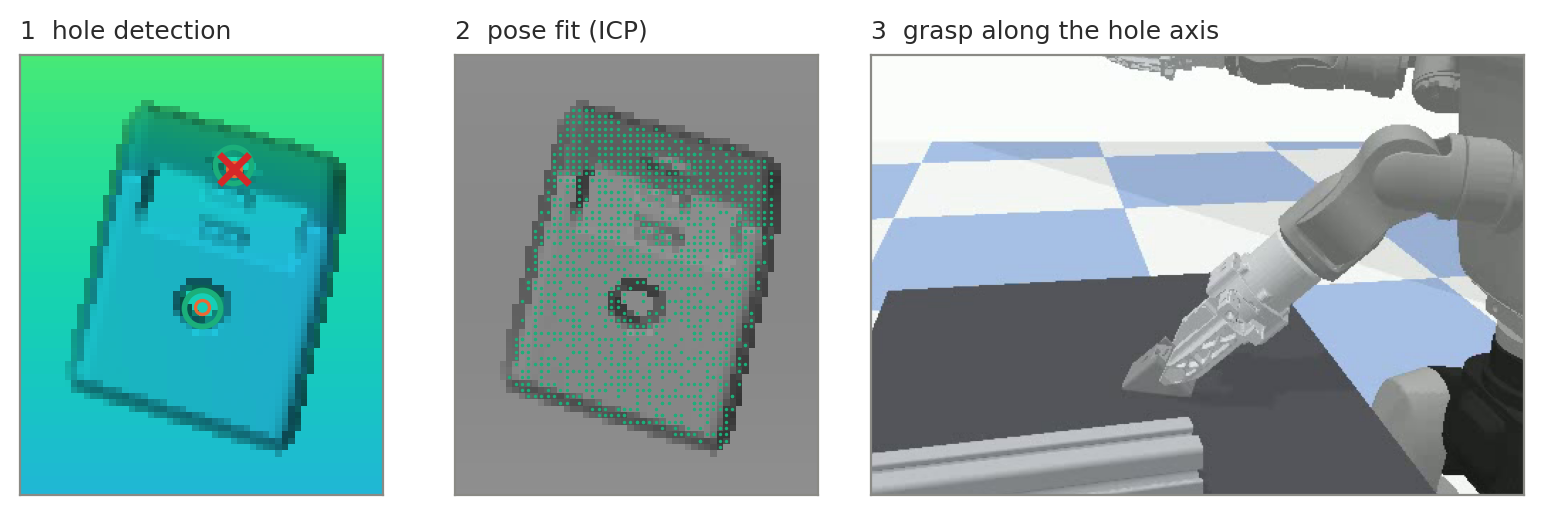
\includegraphics[width=0.85\linewidth]{tasks.png}
\caption{The three stages on ideal depth (seed 204). Detection: hole candidates (orange), true openings
(green rings) and the chosen top hole (red $\times$). Pose fit: the fitted CAD model's visible points. Grasp:
the jaws approach along the hole axis.}
\label{fig:tasks}
\end{figure}

\paragraph{A stand-in for a learned model.} In a real cell this step would more likely be a learned pose
estimator or an end-to-end robot policy. We considered a model-based network (FoundationPose), but it needs a
GPU stack and pretrained weights, against the requirement that everything run on a laptop. The geometric
pipeline is a deliberate surrogate for it. It relies on the same depth cues a network uses, whether for pose
estimation or inside a policy: planar faces, depth edges, small holes a few pixels wide, and surface normals.
If the camera model destroys or shifts these cues, a model that depends on them is affected as well. Its
thresholds play the role of learned parameters: tuned on ideal synthetic depth, they behave like the weights
of a network trained only on ideal synthetic data and then deployed on the real sensor. Unlike a network, the
pipeline is transparent, so every failure can be traced to the camera effect that caused it. The limitation is
that a network trained on noisy depth may learn to tolerate some of the effects; the pipeline therefore
measures how sensitive the cues are, not how a particular network would perform.

\begin{figure}[htbp]
\centering
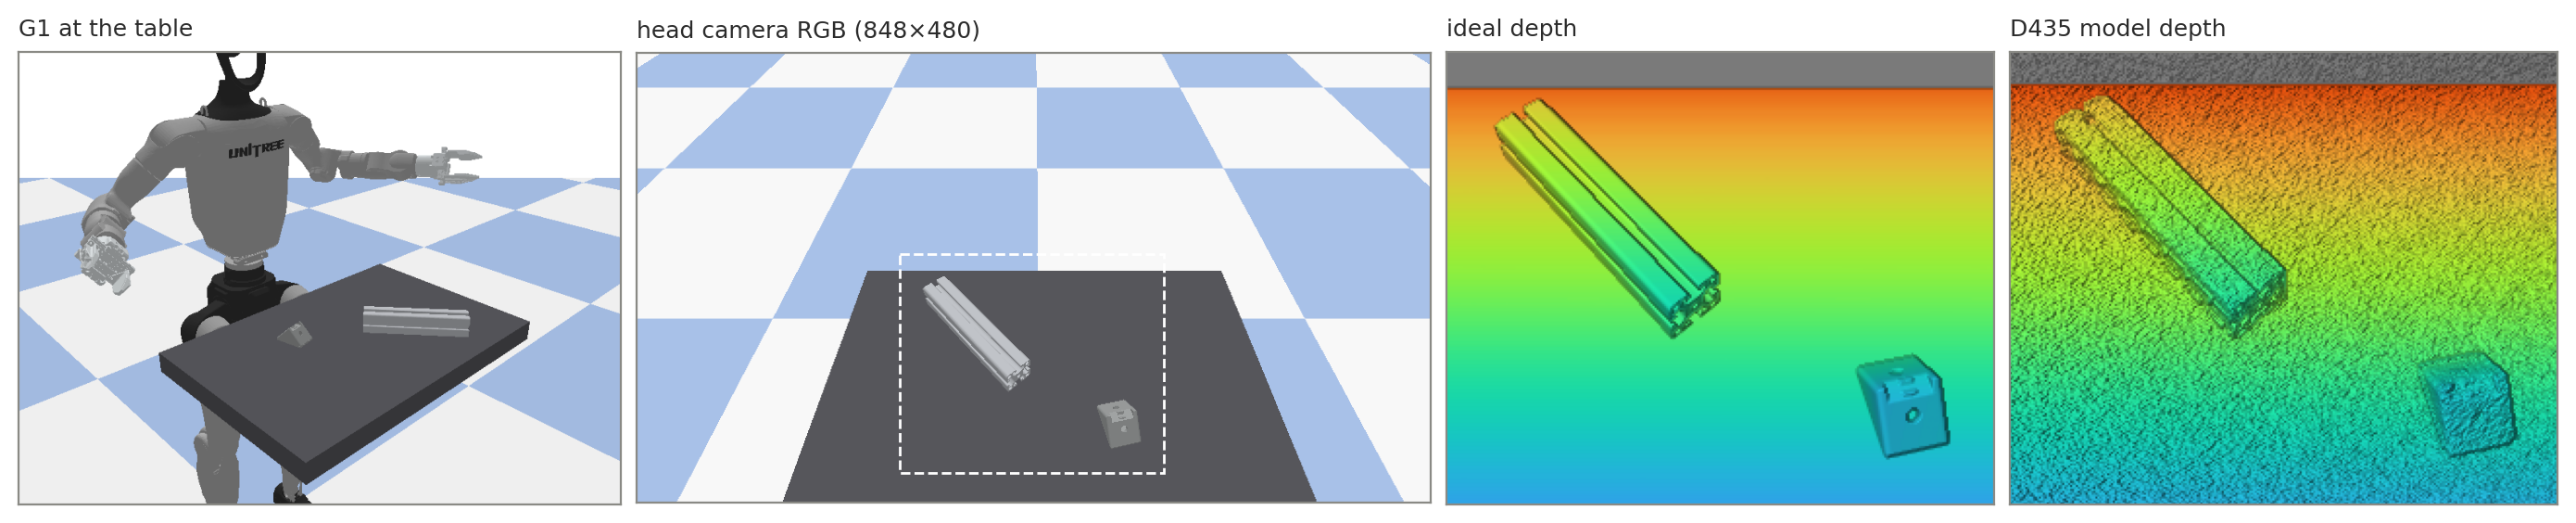
\includegraphics[width=\linewidth]{scene.png}
\caption{The cell and one frame (seed 204). From left: the G1 at the table in its observation pose, the head
camera's RGB image, and the ideal and D435-model depth of the marked region.}
\label{fig:scene}
\end{figure}

% =====================================================================================================
\section{D435 camera model}
\paragraph{Approach.} We corrupt the ideal depth with closed-form models, one effect at a time, so that each
effect can be switched on alone and its downstream consequence measured. A physics-based simulation of the
infrared stereo pair would be more faithful, but the D4 matcher's parameters are undocumented and the
simulation would itself need validation against real data. Learned noise models need real D435 depth of
similar scenes; we found no released D435 noise generator. The scope rule is that every modelled effect has a
published number, so that the model can be traced to its sources and later calibrated.

\paragraph{Effects included.} The D435 measures disparity $d$ between its two infrared imagers, with baseline
$B = 50$\,mm, and reports depth $Z = fB/d$. Three effects are applied in the order in which they arise in the
camera.
\begin{enumerate}
  \item \emph{Edge fattening.} A stereo matcher compares windows of pixels; at a depth step the window
  straddles both sides and the foreground wins, so the foreground grows into the background and narrow gaps
  close. No value is published for the D435. We use the only measured value, from Intel's previous R200
  camera \cite{keselman}: gaps narrower than 5\,px merge, i.e.\ the foreground grows by 2\,px.
  \item \emph{Axial noise}, added to the disparity of each pixel:
  \begin{equation}
    d' = d + s\,\xi,\quad \xi \sim \mathcal N(0,1)
    \qquad\Rightarrow\qquad
    \sigma_Z \approx \frac{Z^2}{fB}\,s ,
  \end{equation}
  with Intel's subpixel accuracy $s = 0.08$\,px \cite{bkm}, giving $\sigma_Z = 0.9$\,mm at 0.5\,m.
  \item \emph{Depth bias} at the datasheet's accuracy limit of $\pm 2\,\%$: $Z' = (1+b)\,Z$ with
  $b = \pm 0.02$, the sign drawn with equal probability. Since back-projection is linear in $Z$, every 3D point
  moves along its own viewing ray; shapes and orientations are preserved and the part shifts by about 10\,mm.
\end{enumerate}
The datasheet's output rules are applied last: the invalid band at the left image edge, the minimum depth of
195\,mm and the 1\,mm depth unit. Lateral error needs no separate term: in stereo the depth map lies on a
fixed pixel grid, and lateral error arises from the axial noise through back-projection and from edge
fattening at depth steps.

\paragraph{Effects left out.} Several effects do not matter for a static, indoor, single-frame, depth-only
task: temporal noise, rolling shutter and motion blur (the depth imagers have a global shutter), ambient
infrared, interference between cameras, defocus, colour-sensor effects and post-processing filters (off by
default). Dropouts (pixels without depth) are left out for lack of a usable number. The datasheet bounds
them only on its test target: a fill rate of at least 99\,\% on a flat, matte white wall within 2\,m
\cite{d435ds}, with no rule for where invalid pixels occur. At that level they are isolated pixels, which fail
the detector's size and roundness tests. No measurement exists for anodized aluminium; dropout patches on the
profile, where its faces reflect the projector pattern away at steep angles, would add false-hole candidates
on the profile, which the CAD fit already rejects in 99--100\,\% of draws. The bracket is matte
powder-coated, close to the datasheet target, and false depth on the profile's T-slots is rejected the same
way. For the remaining effects no usable number exists: the
dependence on incidence angle (the only published term \cite{ahn} is hand-set and does not reproduce its own
measurements), occlusion shadows inside the image, and the spatially correlated ``egg carton'' noise that
Intel describes without a correlation length.

The noise level itself is uncertain. Ahn et al.\ \cite{ahn} fitted the axial noise of a real D435 to about
2.7 times Intel's value at 0.5\,m, still within the range Intel measures on different surfaces (0.07--0.32\,px).
On the development scenes this level alone collapses the pipeline (CAD fit in 4 of 150 draws, against 143 with
Intel's value), so the published noise level decides between a working and a failing perception stage.

% =====================================================================================================
\section{Experiment: does the camera model change the downstream outcome?}
The experiment asks whether the camera model changes the outcome of the three stages of
Section~\ref{sec:pipeline}: hole detection, CAD fit and grasp. The detector's thresholds lie at the D435's
noise level ($\sigma_Z \approx 0.9$\,mm), so an effect of the noise on detection is expected.

\paragraph{Protocol.} The pipeline, the camera model and the hypotheses were developed on 15 scenes, which
were then closed. The test protocol was fixed before any test run (git tag \texttt{final-experiment}). The
30 test scenes are the first seeds from 201 on for which every stage succeeds with ideal depth, so that every
failure is caused by the camera model. Seven depth conditions are compared: ideal, datasheet rules only, each
effect alone, edge fattening with axial noise, and the full model. Each scene is run with 5 noise draws that
are paired across conditions (same random numbers and bias sign), giving 150 draws per condition, compared
with ideal by an exact McNemar test. Because the bias moves every position by about 10\,mm, detection and
pose count as correct within 15\,mm; the strict 3\,mm and 5\,mm criteria are reported as accuracy.

\paragraph{Results.} Table~\ref{tab:results} and Fig.~\ref{fig:results} summarise the sweep.
% TODO: verdict per hypothesis, if wanted as a list
The datasheet rules leave perception unchanged (below 1\,mm) but lower the grasp to 77\,\%: the 1\,mm
rounding nudges the fitted pose, and the grasp search switches to a candidate the arm cannot reach. This row is
the control for the grasp planner's own sensitivity, against which the camera effects on the grasp should be
read. Axial noise causes the largest single drop in detection, to 56\,\%: it leaves enclosed gaps on the
profile's flat top face that pass as holes, and it breaks up the bracket's faces so that the real hole is no
longer enclosed (Fig.~\ref{fig:holeplane}). Edge fattening alone does not prevent detection, since the plug it puts into the hole still
stands out on noise-free depth, but it tilts the hole axis (0.75$^\circ$ to 1.12$^\circ$) and with noise it
lowers detection further, from 56\,\% to 39\,\% ($p = 0.005$, Fig.~\ref{fig:detection}). The depth bias is
invisible to detection but shifts the whole pose by 10.7\,mm along the viewing ray and lowers the grasp to
66\,\%. The full model degrades every stage. Throughout, the CAD fit absorbs most perception errors, because it
tries every candidate and keeps the one that matches the bracket.

\paragraph{Second renderer.} The sweep was repeated with Isaac Sim RTX depth for the same 30 scenes and
noise draws. Ideal depth again succeeds in every stage. Hole detection reaches 61\,\% with axial noise,
97\,\% with edge fattening, 48\,\% with both ($p = 0.022$ against axial alone), 98\,\% with the bias and
53\,\% with the full model; the pose is found in 99--100\,\% of draws and the bias shifts it by 10.7\,mm, as
with PyBullet. The pattern and the sizes of the effects agree within a few percentage points, so they come
from the camera model and not from the renderer. The grasp runs in PyBullet in both cases and is not an
independent check.

\begin{table}[htbp]
\centering
\begin{tabular}{lccc}
\toprule
Condition & Hole detected & Pose found & Grasp lifted \\
\midrule
ideal & 100\,\% & 100\,\% & 100\,\% \\
datasheet rules & 100\,\% & 100\,\% & 77\,\% \\
axial noise & 56\,\% & 99\,\% & 63\,\% \\
edge fattening & 100\,\% & 100\,\% & 63\,\% \\
edge + axial & 39\,\% & 100\,\% & 65\,\% \\
depth bias $\pm$2\,\% & 100\,\% & 100\,\% (10.7\,mm off) & 66\,\% \\
full model & 54\,\% & 99\,\% (10.9\,mm off) & 57\,\% \\
\bottomrule
\end{tabular}
\caption{Success per stage, 30 test scenes $\times$ 5 paired noise draws. Detection and pose within 15\,mm.}
\label{tab:results}
\end{table}

\begin{figure}[htbp]
\centering
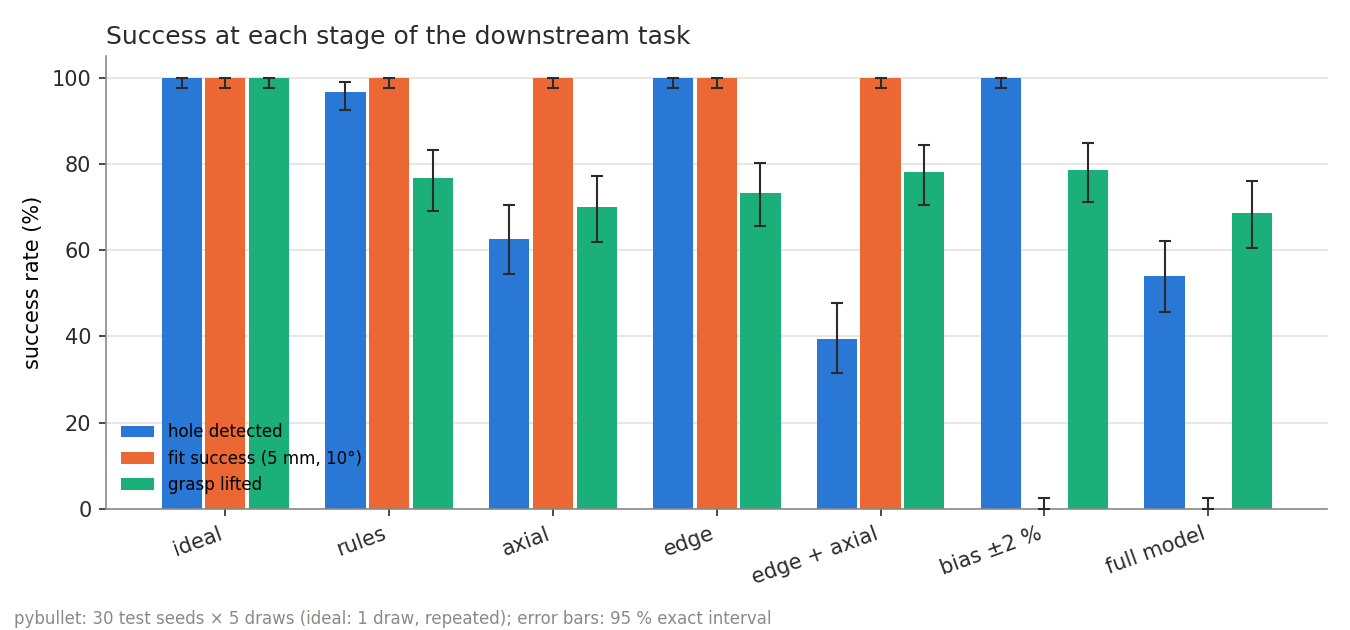
\includegraphics[width=0.85\linewidth]{all_stages.png}
\caption{Success per stage and condition with 95\,\% exact intervals.}
\label{fig:results}
\end{figure}

\begin{figure}[htbp]
\centering
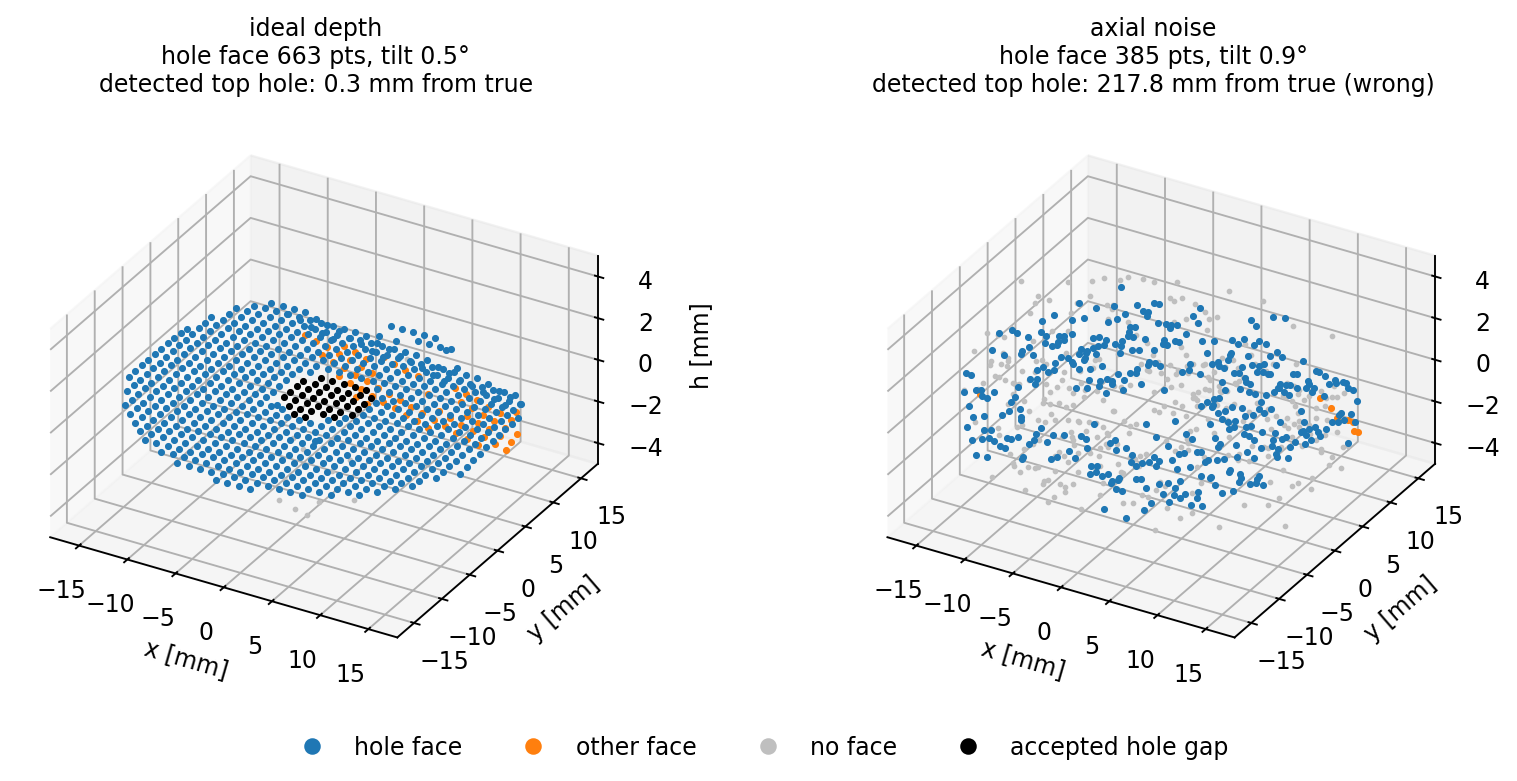
\includegraphics[width=0.8\linewidth]{hole_plane.png}
\caption{Why detection fails under axial noise: depth points within 18\,mm of the true top hole, in the hole's
frame (height $h$ stretched about 4$\times$), coloured by what the detector made of them. With ideal depth the
face is one clean plane and the hole is an enclosed gap (black). With axial noise ($\sigma_Z \approx 0.9$\,mm)
many points fall outside the 1\,mm face band, the face breaks up, no gap is enclosed, and the detector picks a
false hole 218\,mm away. Development scene (seed 8, draw 22).}
\label{fig:holeplane}
\end{figure}

\begin{figure}[htbp]
\centering
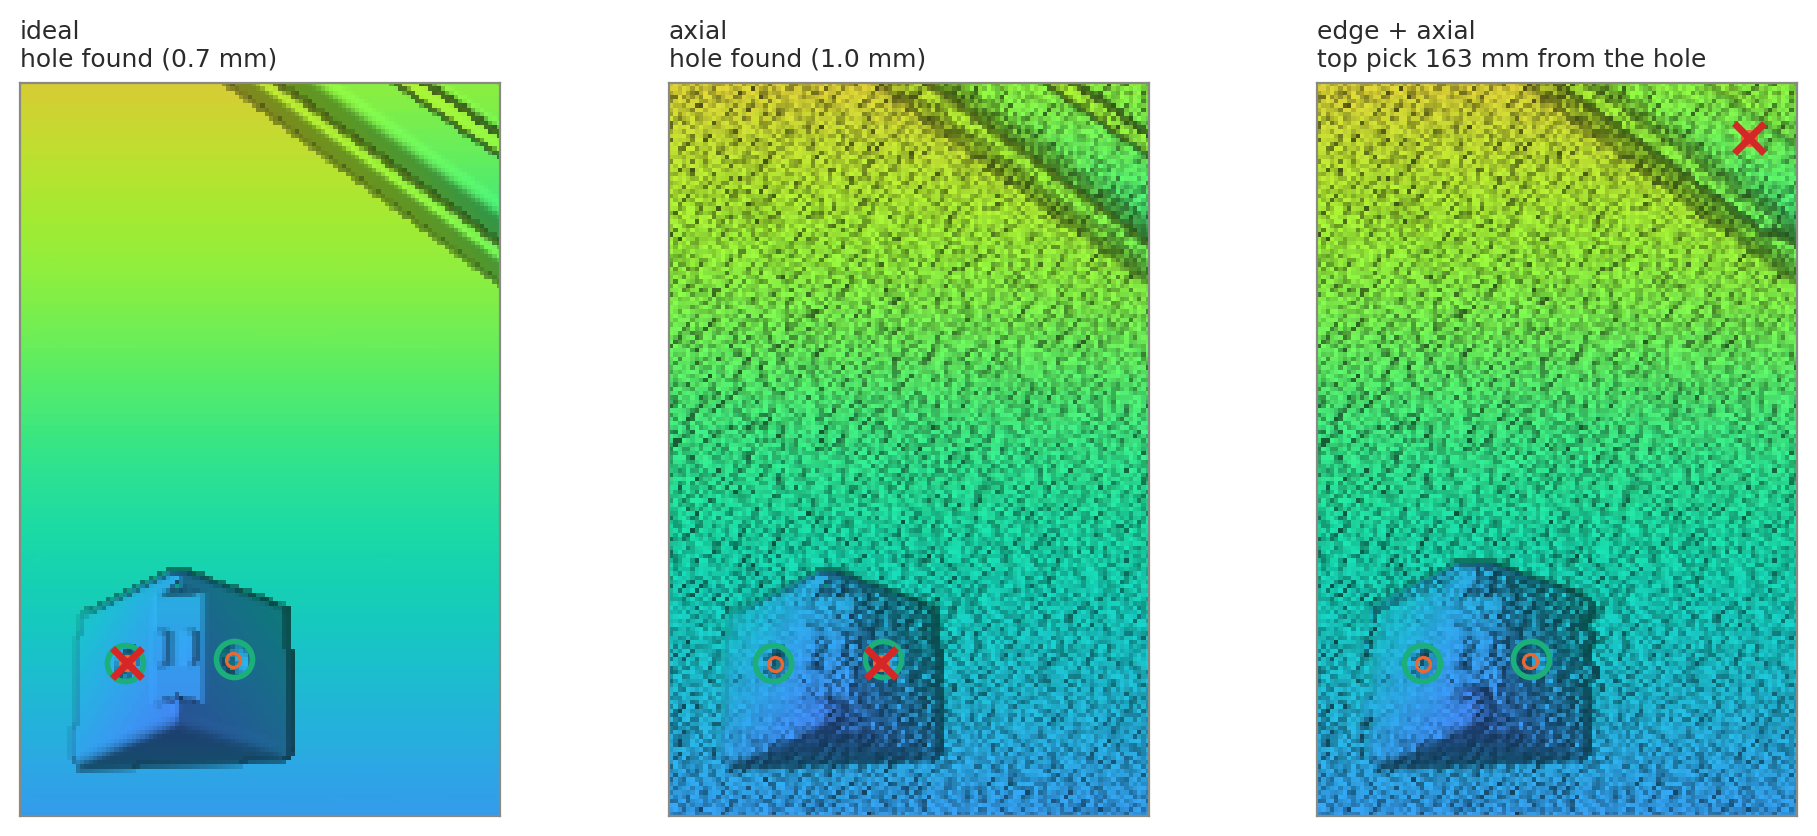
\includegraphics[width=\linewidth]{detection.png}
\caption{The same noise draw (seed 299) under three conditions. Green ring: true top hole; orange: hole
candidates; red cross: the detector's pick. With axial noise the hole is still found; adding edge fattening
fills it, and a false hole on the profile 163\,mm away wins.}
\label{fig:detection}
\end{figure}

\begin{figure}[htbp]
\centering
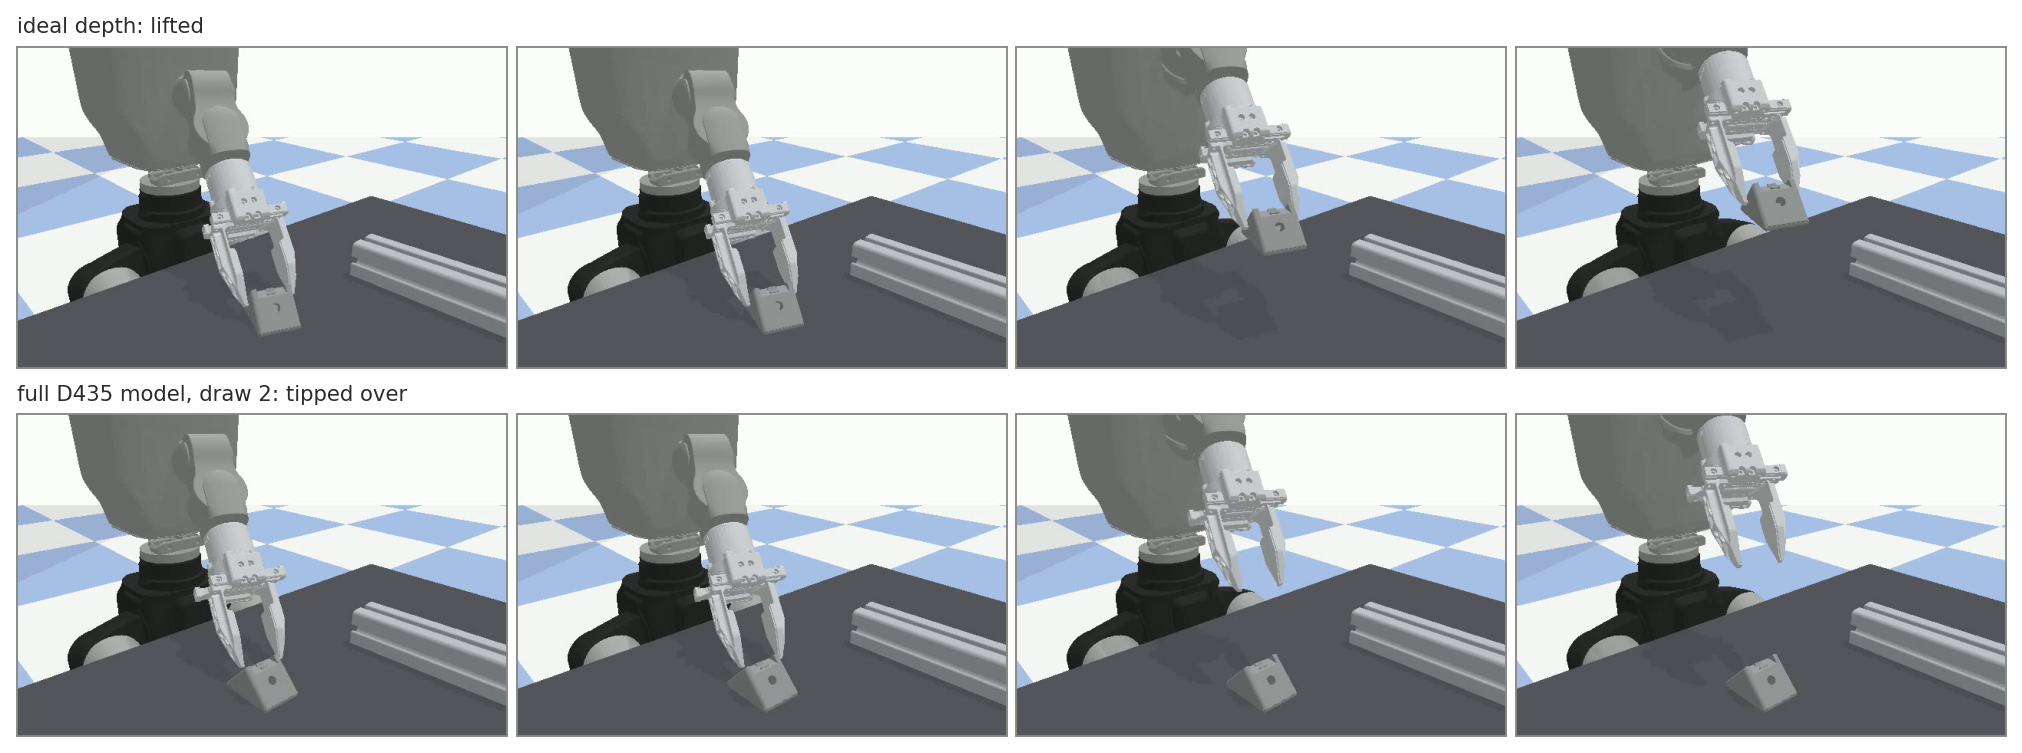
\includegraphics[width=\linewidth]{grasp.png}
\caption{One scene (seed 204) grasped with ideal depth (top) and with the full camera model (bottom, draw 2).
Under the full model every stage degrades: the detector picks a false hole on the profile 161\,mm away, the
CAD fit recovers the bracket but 11.6\,mm off, and the jaws close off-centre and tip the bracket over.}
\label{fig:grasp}
\end{figure}

\paragraph{What did not work.} Three failure patterns remain. When axial noise breaks up every face, there is
no hole candidate and the pipeline stops without a pose. When all candidates are false, the CAD fit can lock
onto the profile (one case 253\,mm and 43$^\circ$ off); the grasp planner then finds no reachable grasp, so the
robot does not move. And near-correct poses still produce failed grasps (Fig.~\ref{fig:grasp}): the planner is
sensitive to millimetre changes. The pipeline also has its own limits, which the test-scene selection hides.
On scenes filtered only for a visible hole, ideal depth reaches 90\,\% detection (the misses pick a round gap
in the bracket's cap) but only 47\,\% grasp success, mostly because the planner tries one grasp candidate and one
hand orientation before reporting an IK failure.

\paragraph{Implications for learned policies.} The two perception stages respond to the camera very
differently. Hole detection depends on a local cue a few pixels wide and drops from 100\,\% to 54\,\% under the
full model. The CAD fit integrates
over the whole visible surface and still finds the bracket in 99\,\% of the cases. This argues against
training an end-to-end policy directly on depth images: such a policy has to read the same local cues, the
hole and the face edges, and would inherit their fragility, while its training data would also have to carry
the right sensor effects. An explicit reconstruction step, model-based fitting such as ICP against CAD or any
other module that recovers the object's state from the whole surface, absorbs most of the sensor error before
the robot acts, and a policy trained on that state sees far less of the sim-to-real gap. It does not remove
everything: a systematic error such as the depth bias passes through the fit as an 11\,mm offset and still
costs grasps. We did not train a policy; this conclusion rests on the contrast between the two stages.

\paragraph{Limitations.} The evaluation is synthetic: it shows how sensitive the pipeline is to the model.
How close the model is to a real D435 is checked in Section~\ref{sec:realism}. The edge-fattening width comes
from the R200, the noise is independent per pixel, there is no angle dependence, and PyBullet renders no
material effects.

% =====================================================================================================
\section{How realistic is the camera model?}
\label{sec:realism}
The model is built from Intel's documentation, not fitted to real data. As a basic check we applied it to
the ground truth of HAMMER \cite{hammer}, which pairs real D435 depth with depth rendered from 3D scans of the
same view (108 frames, 13 indoor scenes, 0.4--1.4\,m; \texttt{camera\_model/validate\_hammer.py},
Fig.~\ref{fig:hammer}). The documented effects appear with similar size: the noise grows with distance as
Intel's formula predicts (2.0 against 1.2\,mm plane residual at 0.53\,m), and the real unit has a scale bias of
$+3.1\,\%$, comparable to our $\pm 2\,\%$. Two effects differ: the real noise is spatially correlated, and at
depth edges the foreground bleeds in only partially (about a third of the pixels, another 40\,\% invalid)
against almost all of them in our model, so our edge fattening is likely too strong. Missing depth (10--40\,\%
of pixels on walls and the dark table), for which the documentation gives no number, is absent from the model.
The check uses one unit and household objects, so it shows the model is of the right kind and size, not that
it predicts real success rates.

\begin{figure}[htbp]
\centering
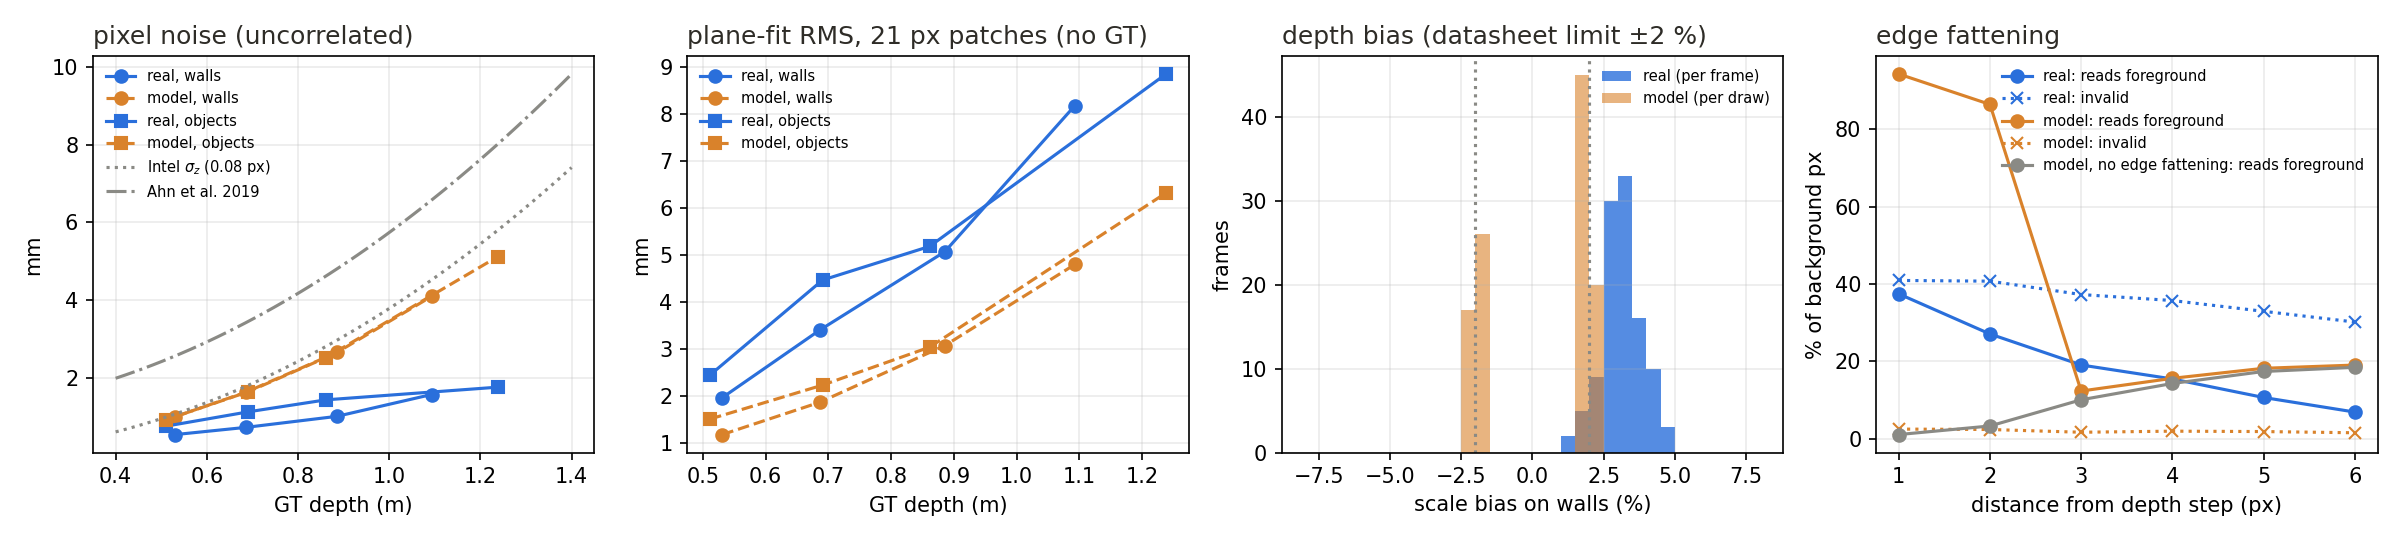
\includegraphics[width=\linewidth]{hammer.png}
\caption{Real D435 depth (HAMMER, blue) against our model applied to HAMMER's ground truth (orange), 108
frames. From left: pixel-to-pixel noise, plane-fit residual in 21$\times$21\,px patches (no ground truth
needed), per-frame scale bias on walls (dotted: datasheet limit $\pm 2\,\%$), and background pixels near depth
steps that read the foreground depth or are invalid.}
\label{fig:hammer}
\end{figure}

% =====================================================================================================
\section{Riskiest sim-to-real assumption (draft)}
% DRAFT: at most one page; to be rewritten by the author. Points collected so far.
A perception model adapts its parameters to the data it was developed on. The baseline detector, tuned on
ideal depth, fails on D435 noise in the same way that a network or a robot policy trained on ideal synthetic
depth would fail on the real camera. Generating the training data through a camera model adapts the
parameters to the sensor that will be deployed: targeted data quality
rather than the broad domain randomisation most sim-to-real approaches rely on, which brings its own
difficulties for training.

The risk is that the adaptation is only as good as the camera model. The two published noise levels for the
D435 differ by a factor of 2.7, and parameters adapted to the lower one meet the higher one as the ideal-tuned
detector met Intel's noise. The riskiest assumption is therefore that the simulated sensor matches the real
one where it matters for the task.
% TODO: state the riskiest assumption in your own words.

\paragraph{First six months (draft).} The work so far suggests measuring before modelling: validate the camera
model against real D435 depth with ground truth, per depth range and separately at edges; calibrate the edge
fattening on the D435 itself; and measure the angle dependence between 60$^\circ$ and 75$^\circ$, where no data
exist.
% TODO: own plan.

% =====================================================================================================
\section*{Use of AI tools}
I used Claude Code throughout. It found, read and summarised the sources (datasheet, tuning guide, papers),
looked up values and page references, and wrote and ran the code under my decisions. It drafted the report's
prose from my notes and decisions; I revised and rewrote every section myself.
I did not read the sources in full myself; instead I had claims checked against the source text, which found
wrong page numbers, a citation attributed to the wrong camera (Keselman's values are for the R200) and a
miscounted result. The main disagreement concerned edge fattening: the AI recommended modelling it with a
swept width from the start and later ranked it first again. I declined, because no D435 value exists and an
invented width would break traceability. In the end I tested it only with the one published number and marked
it as needing calibration. The AI also recommended BlenderProc as the simulator; I chose Isaac Sim for its
physics and robot integration and kept PyBullet so that the work runs on a laptop.

% =====================================================================================================
\begin{thebibliography}{9}
\bibitem{d435ds} Intel, \emph{Intel RealSense D400 Series Datasheet}, rev.\ 017, 2026.
\bibitem{bkm} A. Grunnet-Jepsen, J. N. Sweetser, J. Woodfill, \emph{Best-Known-Methods for Tuning Intel
RealSense D400 Depth Cameras for Best Performance}, Intel, rev.\ 2.0.
\bibitem{keselman} L. Keselman, J. I. Woodfill, A. Grunnet-Jepsen, A. Bhowmik, Intel RealSense Stereoscopic
Depth Cameras, \emph{CVPR Workshops}, 2017.
\bibitem{ahn} M. S. Ahn, H. Chae, D. Noh, H. Nam, D. Hong, Analysis and Noise Modeling of the Intel RealSense
D435 for Mobile Robots, \emph{Int.\ Conf.\ on Ubiquitous Robots (UR)}, 2019.
\bibitem{hammer} H. Jung, P. Ruhkamp, G. Zhai, N. Brasch, Y. Li, Y. Verdie, J. Song, Y. Zhou, A. Armagan,
S. Ilic, A. Leonardis, N. Navab, B. Busam, On the Importance of Accurate Geometry Data for Dense 3D Vision
Tasks, \emph{CVPR}, 2023 (HAMMER dataset).
\end{thebibliography}

\end{document}
